\documentclass[jss]{jss}\usepackage[]{graphicx}\usepackage[]{color}
%% maxwidth is the original width if it is less than linewidth
%% otherwise use linewidth (to make sure the graphics do not exceed the margin)
\makeatletter
\def\maxwidth{ %
  \ifdim\Gin@nat@width>\linewidth
    \linewidth
  \else
    \Gin@nat@width
  \fi
}
\makeatother

\usepackage{Sweave}



%\VignetteEngine{knitr::knitr}
%\VignetteIndexEntry{sparseHessianFD}
%\VignettePackage{sparseHessianFD}

\usepackage{amsmath}
\usepackage{amsfonts}
\usepackage{amsthm}
\usepackage{subcaption}
\usepackage{algorithm}
\usepackage{algorithmic}
\usepackage{tabularx}
\usepackage{dcolumn}
\usepackage{booktabs}
\usepackage{etoolbox}
\usepackage{placeins}
\newtoggle{tikz}
\toggletrue{tikz}


\iftoggle{tikz}{
\usepackage{tikz}
}{}

   \newcolumntype{d}[1]{D{.}{.}{#1}}
%%\newcommand{\pkg}[1]{\emph{#1}}
%%\newcommand{\proglang}[1]{\textsf{#1}}
%%\newcommand{\filename}[1]{\textit{#1}}
%%\newcommand{\code}[1]{\texttt{#1}}
\newcommand{\func}[1]{\code{#1}}
\newcommand{\class}[1]{\textsl{#1}}
\newcommand{\funcarg}[1]{\code{#1}}
\newcommand{\variable}[1]{\code{#1}}
\newcommand{\method}[1]{\func{#1}}

 \newcommand{\df}[3]{\mathsf{d}^{#1}f(#2;#3)}
 \newcommand{\parD}[3]{\mathsf{D}^{#1}_{#2}#3}
\newcommand{\hess}[2]{\mathsf{H}_{#1}#2}
\newcommand{\hessLT}[2]{\mathsf{L}_{#1}#2}
\newcommand{\Mat}[1]{\mathbf{#1}}
\newcommand{\Real}[1]{\mathbb{R}^{#1}}
\newcommand{\Complex}[1]{\mathbb{Z}^{#1}}
\DeclareMathOperator{\Imag}{Im}

\author{Michael Braun\\Edwin L. Cox School of Business\\Southern Methodist University}
\Plainauthor{Michael Braun}
\title{\pkg{sparseHessianFD}: An R Package for Estimating Sparse Hessian Matrices}
\Plaintitle{sparseHessianFD: An R Package for Estimating Sparse Hessian Matrices}
\Shorttitle{sparseHessianFD:  Sparse Hessians}
\Keywords{sparse Hessians, sparsity, computation of Hessians,
  graph coloring, finite differences, differentiation, complex step}
\Address{
  Michael Braun\\
  Edwin L. Cox School of Business\\
  Southern Methodist University\\
  6212 Bishop Blvd.\\
  Dallas, TX 75275\\
  E-mail:  \email{braunm@smu.edu}\\
  URL:  \url{http://www.smu.edu/Cox/Departments/FacultyDirectory/BraunMichael}
}


\Abstract{
  Sparse Hessian matrices occur often
  in statistics, and their fast and accurate estimation can
  improve efficiency of numerical optimization and sampling
  algorithms. By exploiting the known sparsity pattern of a Hessian, methods in the
  sparseHessianFD package require many fewer function or gradient
  evaluations than would be required if the Hessian were treated as
  dense. The package implements established graph coloring and
  linear substitution algorithms that were previously unavailable to
  R users, and is most useful when other numerical,
  symbolic or algorithmic methods are impractical, inefficient or
  unavailable.}


\date{December 22, 2016}

%% need no \usepackage{Sweave.sty}

%%\newenvironment{knitrout}{\begin{figure}}{\end{figure}}
\IfFileExists{upquote.sty}{\usepackage{upquote}}{}
\begin{document}






The Hessian matrix of a log likelihood function or log posterior
density function plays
an important role in statistics.  From a frequentist point of view,
the inverse of the negative Hessian is the asymptotic covariance of
the sampling distribution of a maximum
likelihood estimator.  In Bayesian analysis, when evaluated at the
posterior mode, it is the covariance of a Gaussian approximation to
the posterior distribution.  More broadly, many numerical optimization
algorithms require repeated computation, estimation or approximation
of the Hessian or its inverse; see \citet{NocedalWright2006}.

The Hessian of an objective function with $M$ variables has $M^2$
elements, of which $M(M+1)/2$ are unique.  Thus, the storage
requirements of the Hessian, and computational cost of many linear
algebra operations on it, grow quadratically with the number of
decision variables.   For
applications with hundreds of thousands of variables, computing the
Hessian even once might not be practical under time, storage or
processor constraints.  Hierarchical models, in
which each additional heterogeneous unit is associated with its own subset of
variables, are particularly vulnerable to this curse of dimensionality

However, for many problems, the Hessian is
\emph{sparse}, meaning that the proportion of  ``structural''  zeros
(matrix elements that are always zero, regardless of the value at which
function is estimated) is high.  Consider a log
posterior density in a Bayesian hierarchical
model.  If the outcomes across units are conditionally
independent, the cross-partial derivatives of heterogeneous variables
across units are zero.  As the number of units
increases, the size of the Hessian still grows quadratically, but the number
of \emph{non-zero} elements grows only linearly; the Hessian
becomes increasingly sparse.  The row and column indices of the
non-zero elements comprise the \emph{sparsity pattern} of the Hessian,
and are typically known in advance, before computing the values of
those elements.  \proglang{R} packages such as \pkg{trustOptim}
\citep{R_trustOptim}, \pkg{sparseMVN} \citep{R_sparseMVN} and
\pkg{ipoptr} \citep{R_ipoptr} have the capability to accept Hessians
in a compressed sparse format.

The \pkg{sparseHessianFD} package is a tool for estimating
sparse Hessians numerically, using either finite differences or
complex perturbations of
gradients.  Section~\ref{sec:numdiff} will
cover the specifics, but the basic idea is as follows.  Consider a real-valued
function $f(x)$, its gradient $\nabla{f(x)}$, and its Hessian
$\hess{}{f(x)}$, for $x\in\mathbb{R}^M$.  Define the derivative vector
as the transpose of the gradient, and a vector of partial derivatives, so
${\parD{}{}{f(x)}=\nabla f(x)^\top=\left(\parD{}{1}{},\mathellipsis,\parD{}{M}{}\right)}$.   (Throughout the paper, we will try
to reduce notational clutter by referring to the derivative and
Hessian as $\parD{}{}{}$ and $\hess{}{}$, respectively, without the
$f(x)$ symbol).  Let $e_m$ be a vector of zeros, except with a 1 in the $m$th
element, and let $\delta$ be a sufficiently small scalar
constant. A ``finite difference'' linear approximation to the $m$th column of the Hessian is ${\hess{m}{}\approx\left(\nabla f(x+\delta
  e_m)- \nabla f(x)\right)/\delta}$.  Estimating a dense Hessian in this way involves at least $M+1$ calculations of the
gradient: one for the gradient at $x$, and one after perturbing each
of the $M$ elements of $x$, one at a time. Under certain conditions, a
more accurate approximation is the ``complex step'' method:  $\hess{m}{}\approx\Imag\left(\nabla f(x+i\delta
  e_m)\right)/\delta$, where $i=\sqrt{-1}$ and $\Imag$ returns the
imaginary part of a complex
number \citep{SquireTrapp1998}.  Regardless of the approximation method used, if the Hessian is sparse, most of the
elements are constrained to zero.  Depending
on the sparsity pattern of the Hessian, those constraints may let us recover
the Hessian with fewer gradient evaluations by perturbing multiple
elements of $x$ together.  For some sparsity patterns, estimating a Hessian in
this way can be profoundly efficient.  In fact, for the hierarchical models that we consider in
this paper, the number of gradient evaluations does not increase with
the number of additional heterogeneous units.

The package defines the \class{sparseHessianFD} class, whose initializer
requires the user to provide functions that compute an objective
function, its gradient (as accurately as possible, to machine precision), and the sparsity pattern of its Hessian
matrix. The sparsity pattern (e.g., location of structural
zeros) must be known in advance, and cannot vary across the domain of the
objective function. The only functions and methods of the class that
the end user should need to use are the
initializer, methods that return the Hessian
in a sparse compressed format, and perhaps some utility functions that
simplify the construction of the sparsity pattern.  The class also
defines methods that partition the variables into groups that can be perturbed together in a finite
differencing step, and recovers the elements of the Hessian via linear
substitution.  Those methods perform most of the work, but should be
invisible to the user.

As with any computing method or algorithm, there are boundaries around
the space of applications for which \pkg{sparseHessianFD} is the right
tool for the job. In general, numerical approximations are not ``first
choice'' methods because the result is not exact, so
\pkg{sparseHessianFD} should not be used when the application cannot
tolerate any error, no matter how small.  Also, we admit that some
users might balk at having to provide an exact gradient, even though
the Hessian will be estimated numerically.\footnote{It is possible
  that a gradient that is approximated using a complex step method
  would be precise enough to be useful. A further investigation is
  beyond the scope of this paper.} However, deriving a vector of first
derivatives, and writing \proglang{R} functions to compute them, is a
lot easier than doing the same for a matrix of second derivatives, and
more accurate than computing second-order approximations from the
objective function. Even when we have derived the Hessian
symbolically, in practice it may still be faster to estimate the Hessian
using \pkg{sparseHessianFD} than coding it directly.  These are the
situations in which \pkg{sparseHessianFD} adds the most value to the
statistician's toolbox.

This article proceeds as follows.  First, we present
some background information about numerical differentiation, and
sparse matrices in \proglang{R}, in Section~\ref{sec:background}.  In
Section~\ref{sec:using}, we explain how to use the package.
Section~\ref{sec:algorithms} explains the underlying algorithms, and
Section~\ref{sec:timing} demonstrates the scalability of those algorithms.


\section[Background]{Background}\label{sec:background}

Before describing how to use the package, we
present two short background notes.  The first note is an informal
mathematical explanation of numerical estimation of the Hessian
matrix, with an illustration of how the number of gradient estimates
can be reduced by exploiting the sparsity pattern and symmetric
structure.  This note borrows heavily from, and uses the notation in,
\citet[Chapter 6]{MagnusNeudecker2007}. The
second note is a summary of some of the sparse matrix classes that are
defined in the \pkg{Matrix} package \citep{R_Matrix}, which are used
extensively in \pkg{sparseHessianFD}.

\subsection[Numerical differentiation of sparse Hessians]{Numerical
  differentiation of sparse Hessians}\label{sec:numdiff}

The partial derivative of a real scalar-valued function $f(x)$ with
respect to $x_j$ (the $j$th
component of $x\in\Real{M}$) is defined as
\begin{align}
  \label{eq:defParD}
\parD{}{j}{f(x)}=\lim\limits_{\delta\to 0}\frac{f(x+\delta e_j)-f(x)}{\delta}
\end{align}
For a sufficiently small $\delta$, this definition allows for a
linear approximation to $\parD{}{j}{f(x)}$.  The derivative of $f(x)$
is the vector of all $M$ partial derivatives.
\begin{align}
  \parD{}{}{f(x)}=\left(\parD{}{1}{f(x)},\mathellipsis,\parD{}{M}{f(x)}\right)
  \end{align}
 The \emph{gradient} is defined as $\nabla f(x)=\parD{}{}{f(x)}^\top$.

We define the second-order partial derivative as
\begin{align}
  \label{eq:14}
  \parD{2}{jk}{}=\lim\limits_{\delta\to 0}\frac{\parD{}{j}{f(x+\delta e_k)}-\parD{}{j}{f(x)}}{\delta}
\end{align}
and the Hessian as
\begin{align}
  \label{eq:15}
  \hess{}{f(x)}=
  \begin{pmatrix}
    \parD{2}{11}{}&  \parD{2}{12}{}&  \mathellipsis &  \parD{2}{1M}{}\\
    \parD{2}{21}{}&  \parD{2}{22}{}&  \mathellipsis &  \parD{2}{2M}{}\\
    \vdots&\vdots&&\vdots\\
    \parD{2}{M1}{}&  \parD{2}{M2}{}&  \mathellipsis &  \parD{2}{MM}{}
    \end{pmatrix}
\end{align}

The Hessian is symmetric, so $\parD{2}{ij}{}=\parD{2}{ji}{}$.

\subsubsection[Approximation using finite differences]{Approximation using finite differences} 

To estimate the $m$th column of $\hess{}{}$ using finite differences, we choose a
sufficiently small $\delta$, and compute
\begin{align}
  \label{eq:1}
  \hess{m}{f(x)}&\approx\frac{\parD{}{}{f(x+\delta e_m)}-\parD{}{}{f(x)}}{\delta}
\end{align}

For $M=2$, our estimate of a general $\hess{}{f(x)}$ would be
\begin{align}
  \label{eq:FDhess2}
  \hess{}{f(x)}&\approx
  \begin{pmatrix}
    \parD{}{1}{f(x_1+\delta, x_2)}-\parD{}{1}{f(x_1,x_2)}& \parD{}{1}{f(x_1,x_2+\delta)}-\parD{}{1}{f(x_1,x_2)}\\
        \parD{}{2}{f(x_1+\delta, x_2)}-\parD{}{2}{f(x_1,x_2)}&  \parD{}{2}{f(x_1,x_2+\delta)}-\parD{}{2}{f(x_1,x_2)}
    \end{pmatrix}/\delta
\end{align}

This estimate requires three evaluations of the gradient to get
${\parD{}{}{f(x_1,x_2)}}$, ${\parD{}{}{f(x_1+\delta,x_2)}}$, and
${\parD{}{}{f(x_1,x_2+\delta)}}$.

Now suppose that the Hessian is sparse, and that the off-diagonal
elements are zero.  That means that
\begin{align}
  \parD{}{1}{f(x_1,x_2+\delta)}-\parD{}{1}{f(x_1,x_2)}&=0\label{eq:I1}\\
    \parD{}{2}{f(x_1+\delta,x_2)}-\parD{}{2}{f(x_1,x_2)}&=0\label{eq:I2}
\end{align}
If the identity in Equation~\ref{eq:I1} holds for $x_1$, it must also
hold for $x_1+\delta$, and if Equation~\ref{eq:I2} holds for $x_2$, it
must also hold for $x_2+\delta$.  Therefore,
\begin{align}
  \label{eq:FDhess2sp}
  \hess{}{f(x)}&\approx
  \begin{pmatrix}
    \parD{}{1}{f(x_1+\delta, x_2+\delta)}-\parD{}{1}{f(x_1,x_2)}&0\\
        0&  \parD{}{2}{f(x_1+\delta,x_2+\delta)}-\parD{}{2}{f(x_1,x_2)}
    \end{pmatrix}/\delta
\end{align}

Only two gradients,
${\parD{}{}{f(x_1,x_2)}}$ and ${\parD{}{}{f(x_1+\delta,x_2+\delta)}}$,
are needed.
Being able to reduce the number of gradient evaluations from 3 to 2 depends on knowing that
the cross-partial derivatives are zero.

\subsubsection[Approximation using complex steps]{Approximation using complex steps}

If $f(x)$ is defined over a complex domain and is holomorphic, then we
can we can approximate $\parD{}{}{f(x)}$
and $\hess{}{f(x)}$ at real values of $x$ using the complex step
method. This method comes from a Taylor
series expansion of $f(x)$ in the imaginary direction of the complex
plane \citep{SquireTrapp1998}.  After rearranging terms, and taking the imaginary
parts of both sides,
\begin{align}
  \label{eq:complexTaylor}
  f(x+i\delta)&=f(x) + i\delta\parD{}{}{f(x)}+\mathcal{O}(\delta^2)\\
  \parD{}{}{f(x)}&\approx\frac{\Imag(f(x+i\delta))}{\delta}
\end{align}

Estimating a first derivative using the complex step method does not
require a differencing operation, so there is no subtraction operation
that might generate roundoff errors.  Thus, the approximation can be
made arbitrarily precise as $\delta\rightarrow 0$ \citep{LaiCrassidis2008}.  This is not the
case for second-order approximations of
the Hessian \citep{AbreuStich2013}.  However, when the gradient can be
computed exactly, we can compute a first-order approximation to
Hessian by treating it as the Jacobian of
a vector-valued function \citep{LaiCrassidis2008}.

\begin{align}
  \label{eq:CShess2}
  \hess{}{f(x)}&\approx
  \begin{pmatrix}
    \Imag(\parD{}{1}{f(x_1+i\delta, x_2)})& \Imag(\parD{}{1}{f(x_1,x_2+i\delta)})\\
        \Imag(\parD{}{2}{f(x_1+i\delta, x_2)})&\Imag(\parD{}{2}{f(x_1,x_2+i\delta)})
    \end{pmatrix}/\delta
\end{align}

If this matrix were dense, we would need two evaluations of the
$\parD{}{}f(x)$ to estimate it.  If the matrix were sparse, with the same sparsity
pattern as the Hessian in Equation~\ref{eq:FDhess2sp}, and we
assume that structural zeros remain zero for all
complex $x\in\Complex{M}$, then we need only one evaluation.  Suppose
we were to subtract $\Imag(\parD{}{}{f(x_1,x_2)})$ from each column of
$\hess{}{f(x)}$. When $x$ is real, the imaginary part of the gradient
is zero, so this operation has no effect on the value of the
Hessian. But the sparsity constraints ensure that
the following identities hold all complex $x$.

\begin{align}
  \Imag(\parD{}{1}{f(x_1,x_2+i\delta)}) -\Imag(\parD{}{1}{f(x_1,x_2)})&=0\label{eq:I1c}\\
    \Imag(\parD{}{2}{f(x_1+i\delta,x_2)})-\Imag(\parD{}{2}{f(x_1,x_2)})&=0\label{eq:I2c}
\end{align}

As with the finite difference method, because Equation~\ref{eq:I1c} holds
for $x_1$, it must also hold for $x_1+i\delta$, and because Equation~\ref{eq:I2c} holds
for $x_2$, it must also hold for $x_2+i\delta$. Thus,

\begin{align}
  \label{eq:CShess2sp}
  \hess{}{f(x)}&\approx
  \begin{pmatrix}
    \Imag(\parD{}{1}{f(x_1+i\delta, x_2+i\delta)})&0\\
        0&\Imag(\parD{}{2}{f(x_1+i\delta,x_2+i\delta)})
    \end{pmatrix}/\delta
\end{align}

for real $x$.  Only one evaluation of the gradient is required.

\subsubsection[Perturbing groups of variables]{Perturbing groups of variables}

\Citet{CurtisPowellReid1974} describe a method of estimating sparse
Jacobian matrices by perturbing groups of variables together.
\Citet{PowellToint1979} extend this idea to the
general case of sparse Hessians.  This method partitions
the decision variables into $C$ mutually exclusive groups so that the number of gradient
evaluations is reduced.  Define $\Mat{G}\in\Real{M\times C}$ where $\Mat{G}_{mc}=\delta$ if variable $m$ belongs to group $c$, and zero
otherwise.  Define $\Mat{G}_c\in\Real{M}$ as the $c$th column of $\Mat{G}$.

Next, define $\Mat{Y}\in\Real{M\times C}$ such that each column is
either a difference in gradients, or the imaginary part of a
complex-valued gradient, depending on the chosen method.
\begin{align}
  \label{eq:Yg}
  \Mat{Y}_c&=
           \begin{cases}  
             \nabla f(x+G_c)-\nabla f(x)&\text{finite difference method}\\
             \Imag(\nabla f(x+iG_c))&\text{complex step method}
             \end{cases}
\end{align}

If $C=M$, then $\Mat{G}$ is a diagonal matrix with $\delta$ in each
diagonal element.  The matrix equation $\hess{}{}\Mat{G}=\Mat{Y}$ represents the linear approximation
$\hess{im}{}\delta\approx y_{im}$, and we can solve for all elements of $\hess{}{}$
just by computing $\Mat{Y}$. But if $C<M$,
there must be at least one $\Mat{G}_c$ with $\delta$ in at least two
rows. The corresponding column $\Mat{Y}_c$ is computed by perturbing multiple variables at
once, so we cannot solve for any $\hess{im}{}$
without further constraints.

These constraints come from the sparsity pattern and symmetry
of the Hessian. Consider an example with the following values and
sparsity pattern.
\begin{align}
  \label{eq:7}
 \hess{}{f(x)}= \begin{pmatrix}
    h_{11}&0&h_{31}&0&0\\
    0&h_{22}&0&h_{42}&0\\
    h_{31}&0&h_{33}&0&h_{53}\\
    0&h_{42}&0&h_{44}&0\\
    0&0&h_{53}&0&h_{55}
  \end{pmatrix}
\end{align}

Suppose $C=2$, and define group membership of the five variables through the following $\Mat{G}$ matrix.
\begin{align}
  \label{eq:7}
 \Mat{G}^\top= \begin{pmatrix}
 \delta&\delta&0&0&\delta\\
 0&0&\delta&\delta&0
 \end{pmatrix}
\end{align}
Variables 1, 2 and 5 are in group 1, while variables 3 and 4 are in
group 2.

Next, compute the columns of $\Mat{Y}$ using Equation~\ref{eq:Yg}.  We now
have the following system of linear equations from $\hess{}{}\Mat{G}=\Mat{Y}$.
\begin{align}
  \label{eq:11}
  \begin{aligned}[c]
  h_{11}&=y_{11}\\
  h_{22}&=y_{21}\\
  h_{31}+h_{53}&=y_{31}\\
  h_{42}&=y_{41}\\
  h_{55}&=y_{51}\\
  \end{aligned}
  \qquad
  \begin{aligned}[c]
  h_{31}&=y_{12}\\
  h_{42}&=y_{22}\\
  h_{33}&=y_{32}\\
  h_{44}&=y_{42}\\
  h_{53}&=y_{52}
  \end{aligned}
\end{align}
Note that this system is overdetermined.  Both $h_{31}=y_{12}$ and $h_{53}=y_{52}$
can be determined directly, but $h_{31}+h_{53}=y_{31}$ may not
necessarily hold, and $h_{42}$
could be either $y_{41}$ or $y_{22}$.  \Citet{PowellToint1979} prove
that it is sufficient to solve $\hessLT{}{}\Mat{G}=\Mat{Y}$ instead
via a substitution method, where $\hessLT{}{}$ is the lower
triangular part of $\hess{}{}$.  This has the effect of removing the equations
$h_{42}=y_{22}$ and $h_{31}=y_{12}$ from the system, but retaining
$h_{53}=y_{52}$.  We can then solve for
$h_{31}=y_{31}-y_{52}$. Thus, we have determined a
$5\times 5$ Hessian with only three gradient evaluations, in
contrast with the six that would have been needed had $\hess{}{}$ been treated
as dense.

The \pkg{sparseHessianFD} algorithms assign variables to groups
before computing the values of the Hessian.  This is why the sparsity
pattern needs to be provided in advance.  If a non-zero element is
omitted from the sparsity pattern, the resulting estimate of the
Hessian will be incorrect.  The only problems with erroneously including a zero
element in the sparsity pattern are a possible lack of efficiency
(e.g., an increase in the number of gradient evaluations), and that
the estimated value might be close to, but not exactly, zero. The
algorithms for assigning decision variables to groups, and for
extracting nonzero Hessian elements via substitution, are described in
Section~\ref{sec:algorithms}.

\subsection[Sparse matrices in R]{Sparse matrices and the \pkg{Matrix}
  package}\label{sec:Rsparse}

The \pkg{sparseHessianFD} package uses the sparse matrix classes that are defined
in the \pkg{Matrix} package \citep{R_Matrix}.  All of these classes are subclasses of
\class{sparseMatrix}. Only the row and column
indices (or pointers to them), the non-zero values, and some
meta-data, are stored; unreferenced elements are assumed to be
zero. Class names, summarized in Table~\ref{tab:MatrixClasses}, depend on the data type, matrix structure,
and storage format. Values in numeric and logical matrices correspond to the
\proglang{R} data types of the same names.  Pattern matrices contain
row and column information for the non-zero elements, but no
values. The storage format refers to the internal ordering of the
indices and values, and the layout defines a matrix as symmetric (so
duplicated values are stored only once), triangular, or general.  The
levels of these three factors determine the prefix of letters in each
class name. For example, a triangular sparse matrix of numeric (double
precision) data, stored in
column-compressed format, has a class \class{dtCMatrix}.

\begin{table}[tbh]\centering
  \begin{tabular}{ll|ccc}
      \toprule
   Storage&Layout&\multicolumn{3}{c}{Data type}\\
    &&numeric&logical&pattern\\
    \midrule
    Triplet&general&\class{dgTMatrix}&\class{lgTMatrix}&\class{ngTMatrix}\\
    &triangular&\class{dtTMatrix}&\class{ltTMatrix}&\class{ntTMatrix}\\
      &symmetric&\class{dsTMatrix}&\class{lsTMatrix}&\class{nsTMatrix}\\
    \midrule
        Row-compressed&general&\class{dgRMatrix}&\class{lgRMatrix}&\class{ngRMatrix}\\
    &triangular&\class{dtRMatrix}&\class{ltRMatrix}&\class{ntRMatrix}\\
      &symmetric&\class{dsRMatrix}&\class{lsRMatrix}&\class{nsRMatrix}\\
    \midrule
            Column-compressed&general&\class{dgCMatrix}&\class{lgCMatrix}&\class{ngCMatrix}\\
    &triangular&\class{dtCMatrix}&\class{ltCMatrix}&\class{ntCMatrix}\\
      &symmetric&\class{dsCMatrix}&\class{lsCMatrix}&\class{nsCMatrix}\\
\bottomrule
  \end{tabular}
    \caption{Class names for sparse matrices, as defined in the
    Matrix package.}\label{tab:MatrixClasses}
\end{table}

\pkg{Matrix} also defines some other classes of
sparse and dense matrices that we will not discuss here. The
\pkg{Matrix} package uses the \func{as} function to convert sparse
matrices from one format to another, and to convert a \pkg{base}
\proglang{R} matrix to one of the \pkg{Matrix} classes.

The distinctions among sparse matrix classes is important because
\pkg{sparseHessianFD}'s \method{hessian} method returns a
\class{dgCMatrix}, even though the Hessian is symmetric. Depending on how the
Hessian is used, it might be useful to coerce the Hessian into a
\class{dsCMatrix} object.  Also, the utility functions in Table~\ref{tab:helpers} expect or return certain classes of matrices, so
some degree of coercion of input and output might be
necessary. Another useful \pkg{Matrix} function is \func{tril}, which
extracts the lower triangle of a general or symmetric matrix.


\section[Using the package]{Using the package}\label{sec:using}

In this section, we demonstrate how to use the \pkg{sparseHessianFD},
using a hierarchical binary choice model as an example.  Then, we
discuss the sparsity pattern of the Hessian, and estimate the Hessian values.

\subsection[Example: hierarchical binary choice]{Example model: hierarchical binary choice}\label{sec:example}

Suppose we have a dataset of $N$ households, each with $T$
 opportunities to purchase a particular product.  Let $y_i$ be the
 number of times household $i$ purchases the product, out of the $T$
 purchase opportunities, and let $p_i$ be the probability of
 purchase.  The heterogeneous parameter $p_i$ is the same for all $T$
 opportunities, so $y_i$ is a binomial random variable.

 Let $\beta_i\in\Real{k}$ be a heterogeneous coefficient vector that
 is specific to household $i$, such that
 $\beta_i=(\beta_{i1},\dotsc,\beta_{ik})$. Similarly,
 $z_i\in\Real{k}$ is a vector of household-specific covariates. Define each
 $p_i$ such that the log odds of $p_i$ is a linear function of
 $\beta_i$ and $z_i$, but does not depend directly on $\beta_j$ and $z_j$ for
 another household $j\neq i$.
\begin{align}
  p_i=\frac{\exp(z_i'\beta_i)}{1+\exp(z_i'\beta_i)},~i=1 ... N
\end{align}

The coefficient vectors $\beta_i$ are distributed across the population of households
following a multivariate normal distribution with mean $\mu\in\Real{k}$ and
covariance $\Mat{\Sigma}\in\Real{k\times k}$.   Assume that we know
$\Mat{\Sigma}$, but not $\mu$, so we place a multivariate normal prior
on $\mu$, with mean $0$ and
covariance $\Mat{\Omega}\in\Real{k\times k}$.  Thus, the parameter
vector $x\in\Real{(N+1)k}$ consists of the $Nk$ elements in the $N$ $\beta_i$ vectors,
and the $k$ elements in $\mu$.

The log posterior density, ignoring any normalization constants, is
\begin{align}
  \label{eq:LPD}
  \log \pi(\beta_{1:N},\mu|\Mat{Y}, \Mat{Z}, \Mat{\Sigma},\Mat{\Omega})=\sum_{i=1}^N\left(p_i^{y_i}(1-p_i)^{T-y_i}
  -\frac{1}{2}\left(\beta_i-\mu\right)^\top\Mat{\Sigma}^{-1}\left(\beta_i-\mu\right)\right)
-\frac{1}{2}\mu^\top\Mat{\Omega}^{-1}\mu
\end{align}



\subsection[Sparsity patterns]{Sparsity patterns}\label{sec:sparsity}





Let $x_1$ and $x_2$ be two subsets of elements of $x$.
Define $\parD{2}{x_1,x_2}$ as the product set of cross-partial
derivatives between all elements in $x_1$ and all elements in $x_2$.
Furthermore, define an indexing function Ind$(x_i)$ that returns the
indices in the parameter vector
$x$ that correspond to the elements in $x_i$, and $\hess{x_1,x_2}{}$
as the Hessian elements in rows Ind$(x_1)$ and columns Ind$(x_2)$, and
in rows Ind$(x_2)$ and columns Ind$(x_1)$ (from the symmetry of the
Hessian).

From the log posterior density in Equation~\ref{eq:LPD}, we can see
that $\parD{2}{\beta_i, \beta_i}\neq 0$ (one element of $\beta_i$ could be
correlated with another element of $\beta_i$), and that, for all $i$,
$\parD{2}{\beta_i, \mu}\neq 0$ (because $\mu$ is the prior mean of each
$\beta_i$).  However, since the $\beta_i$ and $\beta_j$ are independently distributed, and the $y_i$ are
conditionally independent, the cross-partial derivatives
$\parD{2}{\beta_i, \beta_j}=0$ for all $i\neq j$. When $N$ is much
greater than $k$, there will be many more zero cross-partial
derivatives than non-zero.  Regardless of how each $\parD{2}{}$ is
mapped to $\hess{}{}$ through the indexing function, the Hessian of the log
posterior density will be sparse.

The sparsity pattern depends on the indexing function; that is, on how the variables are
ordered in $x$. One such ordering is to group all of the
coefficients in the $\beta_i$ for each unit together.
\begin{align}
\beta_{11},\dotsc,\beta_{1k},\beta_{21},\dotsc,\beta_{2k},~\dotsc~,\beta_{N1},\dotsc,\beta_{Nk},\mu_1,\dotsc,\mu_k
\end{align}
In this case, the Hessian has a ``block-arrow'' structure.  For example,
if $N=5$ and $k=2$, then there are 12 total
variables, and the Hessian will have the pattern in Figure~\ref{fig:blockarrow}.

Another possibility is to group coefficients for each covariate
together.
\begin{align}
\beta_{11},\dotsc,\beta_{N1},\beta_{12},\dotsc,\beta_{N2},~\dotsc~,\beta_{1k},\dotsc,\beta_{Nk},\mu_1,\dotsc,\mu_k
\end{align}
Now the Hessian has an "banded" sparsity pattern, as in Figure~\ref{fig:banded}.
\begin{figure}[tbp]
  \begin{subfigure}[b]{.5\textwidth}
\begin{Schunk}
\begin{Soutput}
                             
 [1,] | | . . . . . . . . | |
 [2,] | | . . . . . . . . | |
 [3,] . . | | . . . . . . | |
 [4,] . . | | . . . . . . | |
 [5,] . . . . | | . . . . | |
 [6,] . . . . | | . . . . | |
 [7,] . . . . . . | | . . | |
 [8,] . . . . . . | | . . | |
 [9,] . . . . . . . . | | | |
[10,] . . . . . . . . | | | |
[11,] | | | | | | | | | | | |
[12,] | | | | | | | | | | | |
\end{Soutput}
\end{Schunk}
\caption{A ``block-arrow'' sparsity pattern.}\label{fig:blockarrow}
\end{subfigure}
\begin{subfigure}[b]{.5\textwidth}
\begin{Schunk}
\begin{Soutput}
                             
 [1,] | . . . . | . . . . | |
 [2,] . | . . . . | . . . | |
 [3,] . . | . . . . | . . | |
 [4,] . . . | . . . . | . | |
 [5,] . . . . | . . . . | | |
 [6,] | . . . . | . . . . | |
 [7,] . | . . . . | . . . | |
 [8,] . . | . . . . | . . | |
 [9,] . . . | . . . . | . | |
[10,] . . . . | . . . . | | |
[11,] | | | | | | | | | | | |
[12,] | | | | | | | | | | | |
\end{Soutput}
\end{Schunk}
\caption{A ``banded'' sparsity pattern.}\label{fig:banded}
\end{subfigure}
\caption{Two examples of sparsity patterns for a hierarchical model.}\label{fig:patterns}
\end{figure}

In both cases, the number of non-zeros is the same.   There are
144 elements in this symmetric matrix, but only 64 are
non-zero, and only 38 values are unique.  Although the reduction in
RAM from using a sparse matrix structure for the Hessian may be
modest, consider what would happen if $N=1,000$ instead.  In that case,
there are 2,002 variables in the problem, and more than $4$ million
elements in the Hessian.  However, only $12,004$ of those elements are
non-zero.  If we work with only the lower triangle of the Hessian, then we need to work with
only 7,003 values.

The sparsity pattern required by \pkg{sparseHessianFD} consists of the row and column
indices of the non-zero elements in the \emph{lower triangle} the
Hessian, and it is the responsibility of the user to ensure that
the pattern is correct.  In practice, rather than trying to keep track of the row and column indices
directly, it might be easier to construct a pattern matrix first,
check visually that the matrix has the right pattern, and then extract
the indices.  The package defines utility functions (Table~\ref{tab:helpers}) to convert
between sparse matrices, and the vectors of row and column indices
required by the \class{sparseHessianFD} initializer.

\begin{table}[ptb]
  \centering
  \setlength\extrarowheight{.25em}
  \begin{tabularx}{1.0\linewidth}{lX}
    \toprule
   \func{Matrix.to.Coord} & Returns a list of vectors containing row
                            and column indices of the non-zero
                            elements of a matrix.\\
    \func{Matrix.to.Pointers}&Returns indices and pointers from a
                               sparse matrix.\\
    \func{Coord.to.Pointers}&Converts list of row and column indices
                              (triplet format) to a list of indices
                              and pointers (compressed format).\\
  \bottomrule
  \end{tabularx}
  \caption{sparseHessianFD matrix conversion functions.}
  \label{tab:helpers}
\end{table}

The \func{Matrix.to.Coord} function extracts
row and column indices from a sparse matrix. The following code
constructs a logical block diagonal matrix, converts it to a sparse
matrix, and prints the sparsity pattern of its lower triangle.

\begin{minipage}{\columnwidth}
\begin{Schunk}
\begin{Sinput}
R> library("sparseHessianFD")
R> bd <- kronecker(diag(3), matrix(TRUE, 2, 2))
R> Mat <- as(bd, "nMatrix")
R> printSpMatrix(tril(Mat))
\end{Sinput}
\begin{Soutput}
                
[1,] | . . . . .
[2,] | | . . . .
[3,] . . | . . .
[4,] . . | | . .
[5,] . . . . | .
[6,] . . . . | |
\end{Soutput}
\begin{Sinput}
R> mc <- Matrix.to.Coord(tril(Mat))
R> mc
\end{Sinput}
\begin{Soutput}
$rows
[1] 1 2 2 3 4 4 5 6 6

$cols
[1] 1 1 2 3 3 4 5 5 6
\end{Soutput}
\end{Schunk}
\end{minipage}

\vspace{1em}
To check that a proposed sparsity pattern represents the
intended matrix visually, use the \pkg{Matrix} \func{sparseMatrix} constructor.

\begin{Schunk}
\begin{Sinput}
R> pattern <- sparseMatrix(i=mc$rows, j=mc$cols)
R> printSpMatrix(pattern)
\end{Sinput}
\begin{Soutput}
                
[1,] | . . . . .
[2,] | | . . . .
[3,] . . | . . .
[4,] . . | | . .
[5,] . . . . | .
[6,] . . . . | |
\end{Soutput}
\end{Schunk}

If there is uncertainty about whether an element is a structural
   zero or not, one should err on the side of it being non-zero, and
   include that element in the sparsity pattern.
   There might be a loss of efficiency if the element really is a
   structural zero, but the result will still be correct.  All that
   would happen is that the numerical estimate for that element would be zero
   (within machine precision). On the other hand, excluding a non-zero
   element from the sparsity pattern will likely lead to an incorrect
   estimate of the Hessian.



\subsection[The sparseHessianFD class]{The \class{sparseHessianFD} class}

The function \func{sparseHessianFD} is an initializer that returns a reference to a
\class{sparseHessianFD} object.  The initializer determines an
appropriate permutation and partitioning
of the variables, and performs some additional validation tests.  The arguments to the initializer are
described in Table~\ref{tab:init}.

{\setlength{\extrarowheight}{.25em}
\begin{table}[ptb]
\begin{tabularx}{\linewidth}{>{\bfseries}r X}
  \toprule
x& A numeric vector, with length $M$ at which the object will be
  initialized and tested.\\
fn,gr& \proglang{R} Functions that return the value of the
  objective function, and its gradient. The first argument is the numeric
  variable vector.  Other named arguments can be passed to \func{fn}
  and {gr} as well (see the \funcarg{...} argument below).\\
rows, cols& Sparsity pattern: integer vectors of the row and column indices of
  the non-zero elements in the \emph{lower triangle} of the Hessian.\\
delta& The perturbation amount for finite differencing of the
  gradient to compute the Hessian (the $\delta$ in Section~\ref{sec:numdiff}).  Defaults to
  \code{sqrt(.Machine\$double.eps)}.\\
index1& If \variable{TRUE} (the default), \funcarg{row} and \funcarg{col} use one-based
  indexing.  If \variable{FALSE}, zero-based indexing is used.\\
  complex&If \variable{TRUE}, the complex step method is used.
                If \variable{FALSE} (the default), a simple finite
                differencing of gradients is used.\\
...& Additional arguments to be passed to \func{fn} and \func{gr}.\\
 \bottomrule
\end{tabularx}
\caption{Arguments to the sparseHessianFD initializer.}\label{tab:init}
\end{table}
}

To create a \class{sparseHessianFD} object, just call
\func{sparseHessianFD}.  Applying the default values for the optional
arguments, the usage syntax to create a \class{sparseHessianFD} object is
\begin{Schunk}
\begin{Sinput}
obj <- sparseHessianFD(x, fn, gr, rows, cols, ...)
\end{Sinput}
\end{Schunk}
where \funcarg{...} represents all other arguments that are
passed to \funcarg{fn} and \funcarg{gr}.


The \func{fn}, \func{gr} and \func{hessian} methods respectively evaluate the
function, gradient and Hessian at a variable vector $x$.  The
\func{fngr} method returns the function and gradient as a list.  The
\func{fngrhs} method includes the Hessian as well.


\begin{Schunk}
\begin{Sinput}
R> f <- obj$fn(x)
R> df <- obj$gr(x)
R> hess <- obj$hessian(x)
R> fngr <- obj$fngr(x)
R> fngrhs <- obj$fngrhs(x)
\end{Sinput}
\end{Schunk}


\subsection[An example]{An example}\label{sec:exHess}

Now we can estimate the Hessian for the
log posterior density of the model from Section~\ref{sec:example}.
For demonstration purposes, \pkg{sparseHessianFD} includes functions that compute the value
(\func{binary.f}), the gradient (\func{binary.grad}) and the Hessian
(\func{binary.hess}) of this model. We will treat the result from \func{binary.hess} as a
  ``true'' value against which we will compare the numerical
  estimates.

To start, we load the data, set some dimension parameters, set prior
values for $\Mat{\Sigma}^{-1}$ and $\Mat{\Omega}^{-1}$, and simulate a
vector of variables at which to evaluate the function. The \func{binary.f} and \func{binary.grad} functions take the data and
priors as lists.  The \func{data(binary)} call adds the appropriate data
list to the environment, but we need to construct the prior list
ourselves.

\begin{Schunk}
\begin{Sinput}
R> set.seed(123)
R> data("binary")
R> str(binary)
\end{Sinput}
\begin{Soutput}
List of 3
 $ Y: int [1:50] 13 1 18 18 19 6 16 6 5 8 ...
 $ X: num [1:4, 1:50] -0.07926 -0.23018 1.55871 0.00997 0.01828 ...
 $ T: num 20
\end{Soutput}
\begin{Sinput}
R> N <- length(binary[["Y"]])
R> k <- NROW(binary[["X"]])
R> T <- binary[["T"]]
R> nvars <- as.integer(N * k + k)
R> priors <- list(inv.Sigma = rWishart(1, k + 5, diag(k))[,,1],
+   inv.Omega = diag(k))
\end{Sinput}
\end{Schunk}

This dataset represents the simulated choices for $N= 50$ customers
over $T= 20$ purchase opportunties, where the probability of purchase
is influenced by $k= 4$ covariates.

The next code chunk evaluates the ``true'' value, gradient and
Hessian.  The \funcarg{order.row} argument tells the function whether
the variables are ordered by household (\variable{TRUE}) or by covariate
(\variable{FALSE}). If \funcarg{order.row} is \variable{TRUE}, then the Hessian
will have a banded pattern.  If \funcarg{order.row} is \variable{FALSE}, then the
Hessian will have a block-arrow pattern.

\begin{Schunk}
\begin{Sinput}
R> P <- rnorm(nvars)
R> order.row <- FALSE
R> true.f <- binary.f(P, binary, priors, order.row=order.row)
R> true.grad <- binary.grad(P, binary, priors, order.row=order.row)
R> true.hess <- binary.hess(P, binary, priors, order.row=order.row)
\end{Sinput}
\end{Schunk}

The sparsity pattern of the Hessian is specified by two integer
vectors:  one each for the row and column indices of the non-zero
elements of the lower triangule of the Hessian.  For this example, we happen to have a
matrix with the same sparsity pattern
of the Hessian we are trying to compute, so we can use the
\func{Matrix.to.Coord} function to extract the appropriate index
vectors.  In practice, it is more likely that we would need to determine the row
and column indices directly, through our knowledge of the structure of
the problem.  For a hierarchical model, we can create a block-arrow
pattern matrix using either the \func{Matrix::bdiag} or \func{kronecker} functions to
create a block diagonal matrix, and concatenate dense rows and columns to the margins.

\begin{Schunk}
\begin{Sinput}
R> pattern <- Matrix.to.Coord(tril(true.hess))
R> str(pattern)
\end{Sinput}
\begin{Soutput}
List of 2
 $ rows: int [1:1310] 1 2 3 4 201 202 203 204 2 3 ...
 $ cols: int [1:1310] 1 1 1 1 1 1 1 1 2 2 ...
\end{Soutput}
\end{Schunk}

Finally, we create an instance of a \class{sparseHessianFD} object.
Evaluations of the function and gradient using the \method{fn} and
\method{gr} methods will always give the same
results as the true values because they are computed using the same functions.

\begin{Schunk}
\begin{Sinput}
R> obj <- sparseHessianFD(P, fn=binary.f, gr=binary.grad,
+   rows=pattern[["rows"]], cols=pattern[["cols"]],
+   data=binary, priors=priors, order.row=order.row)
R> f <- obj$fn(P)
R> identical(f, true.f)
\end{Sinput}
\begin{Soutput}
[1] TRUE
\end{Soutput}
\begin{Sinput}
R> gr <- obj$gr(P)
R> identical(gr, true.grad)
\end{Sinput}
\begin{Soutput}
[1] TRUE
\end{Soutput}
\end{Schunk}

The default choice of method is \funcarg{complex=FALSE}, so the
evaluation of the Hessian is a finite differenced approximation,
so it is very close to, but not identical to, the true value, in terms
of mean relative difference.



\begin{Schunk}
\begin{Sinput}
R> hs <- obj$hessian(P)
R> mean(abs(hs-true.hess))/mean(abs(hs))
\end{Sinput}
\begin{Soutput}
[1] 2.3357e-09
\end{Soutput}
\end{Schunk}



If \funcarg{complex=TRUE} in the initializer, the call to the \method{hessian} method will
apply the complex step method. To use this method, the functions
passed as \funcarg{fn} and \funcarg{gr} must both
accept a complex argument, and return a complex
result, even though we are differentiating a real-valued function. Although \pkg{base} \proglang{R} supports complex arguments
for most basic mathematical functions, many common functions (e.g.,  \func{gamma}, \func{log1p},
\func{expm1}, and the probability distribution functions) do not have
complex implementations. Furthermore, the complex step method is valid
only if the function is holomorphic. The methods in \class{sparseHessianFD} do
\emph{not} check that this is the case for the function at hand. We convey the
following warning from the documentation of the \pkg{numDeriv} package
\citep{R_numDeriv}, which also implements the complex step method:
``avoid this method if you do not know that your function is
suitable. Your mistake may not be caught and the results will be
spurious.''

Fortunately for demonstration purposes, the log posterior density in
Equation~\ref{eq:LPD} is holomorphic, so we
can estimate its Hessian using the complex step method, and compute
the mean relative difference from the true Hessian.

\begin{Schunk}
\begin{Sinput}
R> obj2 <- sparseHessianFD(P, fn=binary.f, gr=binary.grad,
+   rows=pattern[["rows"]], cols=pattern[["cols"]],
+   complex=TRUE,
+   data=binary, priors=priors, order.row=order.row)
R> hs2 <- obj2$hessian(P)
R> mean(abs(hs2-true.hess))/mean(abs(hs2))
\end{Sinput}
\begin{Soutput}
[1] 8.0555e-17
\end{Soutput}
\end{Schunk}



In short, the complex step method can be more accurate than
finite differencing, but it comes with theoretical and implementation
restrictions that may limit its universality.

\section[Algorithms]{Algorithms}\label{sec:algorithms}

In this section, we explain how \pkg{sparseHessianFD} works. The
algorithms are adapted from \citet{ColemanGarbow1985}, who provided
Fortran implementations as \citet{ColemanGarbow1985b}.  Earlier
versions of \pkg{sparseHessianFD} included licensed copies of the
\citet{ColemanGarbow1985b} code, on which the current version no
longer depends. Although newer partitioning algorithms have been proposed (e.g.,
\citealp{GebremedhinManne2005,GebremedhinTarafdar2009}), mainly in the
context of automatic differentiation, we have chosen to implement
established algorithms that are known to work well, and are likely
optimal for the hierarchical models that many statisticians will encounter.


\subsection[Partitioning the variables]{Partitioning the variables}\label{sec:coloring}

Finding consistent, efficient partitions can be
characterized as a vertex coloring problem from graph theory \citep{ColemanMore1984}.  In this
sense, each variable is a vertex in an undirected graph, and an edge connects two
vertices $i$ and $j$ if and only if ${\hess{ij}{f(x)}\neq 0}$.  The
sparsity pattern of the Hessian is the adjacency matrix of the graph.
By ``color,'' we mean nothing more than group assignment; if a
variable is in a group, then its vertex has the color associated with
that group.  A ``proper'' coloring of a graph is one in which two
vertices with a common edge do not have the same
color. \Citet{ColemanMore1984} define a ``triangular coloring'' as
a proper coloring with the additional condition that common
neighbors of a vertex do not have the same color.  A triangular
coloring is a special case of an ``cyclic coloring,'' in which any cycle in the graph
uses at least three colors \citep{GebremedhinTarafdar2007}.

An ``intersection set'' contains characteristics that are common to two vertices, and
an ``intersection graph'' connects vertices whose intersection set is
not empty.  In our context, the set in question is the row indices of
the non-zero elements in each column of $\hessLT{}{}$.  In the
intersection graph, two vertices are connected if the corresponding
columns in $\hessLT{}{}$ have at least one non-zero element in a common row.

\Citet{PowellToint1979} write that a partitioning is consistent with a
substitution method if and only if no columns
of the of lower triangle of the Hessian that are
in the same group have a non-zero element in the same
row.  An equivalent statement is that no two adjacent vertices in the
intersection graph can have the same color.  Thus, we can partition
the variables by creating a proper coloring of the intersection graph
of $\hessLT{}{}$.

This intersection graph, and the number of colors needed to
color it, are not invariant to
permutation of the rows and columns of $\hess{}{}$.  Let $\pi$
represent such a permutation, and let $\hessLT{\pi}{}$ be the lower
triangle of $\pi\hess{}{}{\pi^\top}$.    \Citet[Theorem
6.1]{ColemanMore1984} show that a coloring is triangular if and only
if it is also a proper coloring of the intersection
graph of $\hessLT{\pi}{}$.  Furthermore,
\citet{ColemanCai1986} prove that a partitioning is consistent with a
substitution method if and only if it is an acyclic coloring of the
graph of the sparsity pattern of the Hessian.   Therefore,
finding an optimal partitioning of the variables involves finding an
optimal combination of a permutation $\pi$, and coloring algorithm
for the intersection graph of $\hessLT{\pi}{}$.

These ideas are illustrated in Figures~\ref{fig:graph1} and
\ref{fig:graph2}.  Figure~\ref{fig:graph1adj} shows the sparsity pattern of the lower triangle of a
Hessian as an adjacency matrix, and Figure~\ref{fig:graph1pic} is the
associated graph with a proper vertex coloring.  Every column (and
thus, every pair of columns) in Figure~\ref{fig:graph1adj} has a non-zero element
in row 7, so there are no non-empty intersection sets across the
columns.  All vertices are connected to each other in the
intersection graph (Figure~\ref{fig:graph1int}), which requires seven colors for a proper coloring.  Estimating a
sparse Hessian with this partitioning scheme would be no more
efficient than treating the Hessian as if it were dense.
\begin{figure}[ptb]
  \begin{subfigure}[b]{.32\textwidth}\centering
  \begin{tabular}{r|ccccccc}
   & 1&2&3&4&5&6&7\\
    \hline
    1& 1&&&&&&\\
    2&1&1&&&&&\\
    3&0&0&1&&&&\\
    4&0&0&1&1&&&\\
    5&0&0&0&0&1&&\\
    6&1&0&0&0&1&1&\\
    7&1&1&1&1&1&1&1
  \end{tabular}
  \caption{Adjacency matrix.}\label{fig:graph1adj}
\end{subfigure}
\begin{subfigure}[b]{.32\textwidth}\centering
\iftoggle{tikz}{
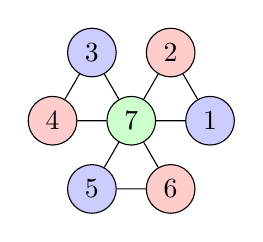
\begin{tikzpicture}
\tikzstyle{every node}=[draw, shape=circle]
\node at (0,0) [fill=green!20] (v7) {7};
\node at (0:1) [fill=blue!20] (v1) {1};
\node at (60:1) [fill=red!20] (v2) {2};
\node at (120:1) [fill=blue!20] (v3) {3};
\node at (180:1) [fill=red!20] (v4) {4};
\node at (240:1) [fill=blue!20] (v5) {5};
\node at (300:1) [fill=red!20] (v6) {6};
\draw
(v1) -- (v7)  (v2) -- (v7)
(v3) -- (v7)  (v4) -- (v7)
(v5) -- (v7)  (v6) -- (v7)
(v1) -- (v2)  (v3) -- (v4)
(v5) -- (v6);
\end{tikzpicture}
}{} %% end toggle
\caption{Sparsity graph.}\label{fig:graph1pic}
\end{subfigure}
\begin{subfigure}[b]{.32\textwidth}\centering
\iftoggle{tikz}{
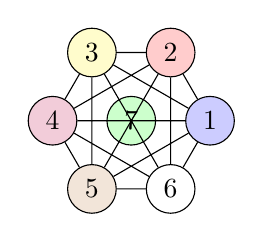
\begin{tikzpicture}
\tikzstyle{every node}=[draw, shape=circle]
\node at (0,0) [fill=green!20] (v7) {7};
\node at (0:1) [fill=blue!20] (v1) {1};
\node at (60:1) [fill=red!20] (v2) {2};
\node at (120:1) [fill=yellow!20] (v3) {3};
\node at (180:1) [fill=purple!20] (v4) {4};
\node at (240:1) [fill=brown!20] (v5) {5};
\node at (300:1) [fill=white!20] (v6) {6};
\draw
(v1) -- (v7)  (v2) -- (v7)  (v3) -- (v7)
(v4) -- (v7)  (v5) -- (v7)  (v6) -- (v7)
(v1) -- (v6)  (v2) -- (v6)  (v3) -- (v6)
(v4) -- (v6)  (v5) -- (v6)
(v1) -- (v5)  (v2) -- (v5)  (v3) -- (v5)
(v4) -- (v5)
(v1) -- (v4)  (v2) -- (v4)  (v3) -- (v4)
(v1) -- (v3)  (v2) -- (v3)
(v1) -- (v2);
\end{tikzpicture}
}{} %% end toggle
\caption{Intersection graph.}\label{fig:graph1int}
\end{subfigure}
\caption{Unpermuted matrix.}\label{fig:graph1}
\end{figure}


Now suppose we were to rearrange $\hess{}{}$ so the last row and
and column were moved to the front.  In Figure~\ref{fig:graph2adj}, all columns share at least one non-zero row with
the column for variable 7, but variable groups $\{2,4,6\}$ and
$\{1,3,5\}$ have empty intersection sets.  The intersection graph in
Figure~\ref{fig:graph2int} has fewer edges than Figure~\ref{fig:graph1int}, and can be colored
with only three colors.
\begin{figure}[ptb]
  \begin{subfigure}[m]{.32\textwidth}\centering
  \begin{tabular}{r|ccccccc}
   & 7&1&2&3&4&5&6\\
    \hline
    7& 1&&&&&&\\
    1&1&1&&&&&\\
    2&1&1&1&&&&\\
    3&1&0&0&1&&&\\
    4&1&0&0&1&1&&\\
    5&1&0&0&0&0&1&\\
    6&1&0&0&0&0&1&1
  \end{tabular}
  \caption{Adjacency matrix.}\label{fig:graph2adj}
\end{subfigure}
\begin{subfigure}[m]{.32\textwidth}\centering
\iftoggle{tikz}{
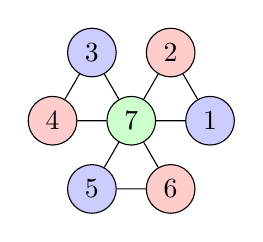
\begin{tikzpicture}
\tikzstyle{every node}=[draw, shape=circle]
\node at (0,0) [fill=green!20] (v7) {7};
\node at (0:1) [fill=blue!20] (v1) {1};
\node at (60:1) [fill=red!20] (v2) {2};
\node at (120:1) [fill=blue!20] (v3) {3};
\node at (180:1) [fill=red!20] (v4) {4};
\node at (240:1) [fill=blue!20] (v5) {5};
\node at (300:1) [fill=red!20] (v6) {6};
\draw
(v1) -- (v7)  (v2) -- (v7)  (v3) -- (v7)
(v4) -- (v7)  (v5) -- (v7)  (v6) -- (v7)
(v1) -- (v2)  (v3) -- (v4)  (v5) -- (v6);
\end{tikzpicture}
}{} %% end toggle
\caption{Sparsity graph.}\label{fig:graph2pic}
\end{subfigure}
\begin{subfigure}[m]{.32\textwidth}\centering
\iftoggle{tikz}{
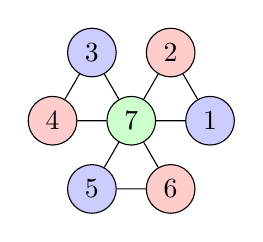
\begin{tikzpicture}
\tikzstyle{every node}=[draw, shape=circle]
\node at (0,0) [fill=green!20] (v7) {7};
\node at (0:1) [fill=blue!20] (v1) {1};
\node at (60:1) [fill=red!20] (v2) {2};
\node at (120:1) [fill=blue!20] (v3) {3};
\node at (180:1) [fill=red!20] (v4) {4};
\node at (240:1) [fill=blue!20] (v5) {5};
\node at (300:1) [fill=red!20] (v6) {6};
\draw
(v1) -- (v7)  (v2) -- (v7)  (v3) -- (v7)
(v4) -- (v7)  (v5) -- (v7)  (v6) -- (v7)
(v1) -- (v2)  (v3) -- (v4)  (v5) -- (v6);
\end{tikzpicture}
}{} %% end toggle
\caption{Intersection graph.}\label{fig:graph2int}
\end{subfigure}
\caption{Permuted matrix.}\label{fig:graph2}
\end{figure}

The practical implication of all of this is that by permuting the
rows and columns of the Hessian, we may be able to reduce the
number of colors needed for a cyclic coloring of the graph of the
sparsity pattern.  Fewer colors means fewer partitions of the
variables, and that means fewer gradient evaluations to
estimate the Hessian.

The \class{sparseHessianFD}
class finds a permutation, and partitions the variables, when it is
initialized. The problem of finding a cyclic
coloring of the graph of the sparsity pattern is NP-complete
\citep{ColemanCai1986}, so the partitioning may not be truly optimal.
Fortunately, we just need the partitioning to be reasonably good, to
make the effort worth our
while.  A plethora of vertex coloring heuristics have been proposed,
and we make no claims that any of the algorithms in \pkg{sparseHessianFD} are even
``best available'' for all situations.

The first step is to permute the rows and columns of the Hessian.   A
reasonable choice is the ``smallest-last'' ordering that
sorts the rows and columns in decreasing order of the number of
elements \citep[Theorem 6.2]{ColemanMore1984}. To justify this permutation, suppose
non-zeros within a row are randomly distributed across
columns.  If the row is near the top of the matrix, there is a higher
probability that any non-zero element is in the upper triangle, not in
the lower.  By putting sparser rows near the bottom, we do not change
the number of non-zeros in the lower triangle, but we should come
close to minimizing the number of non-zeros in each row.  Thus, we
would expect the number of columns with non-zero elements in common
rows to be smaller, and the intersection graph to be sparser \citep{GebremedhinTarafdar2007}.

The adjacency matrix of the intersection graph of the permuted matrix
is the Boolean crossproduct, $\hessLT{\pi}{}^\top \hessLT{\pi}{}$.
Algorithm \ref{alg:coloring} is a ``greedy'' vertex coloring
algorithm, in which vertices are colored sequentially.  The result is
a cyclic coloring on the sparsity graph, which in turn is a consistent
partitioning of the variables.

\begin{algorithm}
  \begin{algorithmic}
    \REQUIRE{$P[i],i=1,\mathellipsis,M$: sets of column indices  of
      non-zero elements in row $i$.}
    \REQUIRE{$F[i],i=1,\mathellipsis,M$:  sets of ``forbidden'' colors for
         vertex $i$ (initially empty)}
    \REQUIRE{$U$:  set of used colors (initially empty)}
    \REQUIRE{$C[i], i=1,\mathellipsis,M$: vector to store output of
      assigned colors (initially all zero)}.
    \STATE{$k\leftarrow 0$} \COMMENT{Largest color index used}
    \STATE{Insert $0$ in $U$}
    \FOR{$i=1$ \TO $M$}
       \IF{$F[i]$ is empty (no forbidden colors)}
           \STATE{$C[i]\leftarrow 0$}
        \ELSE
           \STATE{$V\leftarrow U - F[i]$}\COMMENT{Used colors that are
             not forbidden}
           \IF{$V$ is empty}
              \STATE{$k\leftarrow k+1$}
              \STATE{Insert $k$ into $U$}
              \STATE{$C[i]\leftarrow k$}
        \ELSE
             \STATE{$C[i]\leftarrow\min(V)$}
\COMMENT{Assign smallest existing non-forbidden color to $i$}
             \ENDIF
    \ENDIF
    \ENDFOR
    \FOR{$j$ in $P[i]$}
    \STATE{Insert $C[i]$ into $F[j]$}
\COMMENT{Make $i$'s color forbidden to all of
      its uncolored neighbors}
    \ENDFOR
    \RETURN{$C$}
    \end{algorithmic}
    \caption{Consistent partitioning of variables for a triangular
      substitution method.}\label{alg:coloring}
    \end{algorithm}


\subsection[Computing the Hessian by substitution]{Computing the Hessian by substitution}

The cycling coloring of the sparsity graph defines the $\Mat{G}$
matrix from Section \ref{sec:numdiff}.  We then estimate $\Mat{Y}$
using Equation~\ref{eq:Yg}.   Let $C_m$ be the assigned color to
variable $m$.  The substitution method is defined in
\citet[Equation 6.1]{ColemanMore1984}.
\begin{align}
  \label{eq:subst}
  \hess{ij}{f(x)}&=\Mat{Y}_{i,C_j}/\delta - \sum_{l>i,l\in C_j}\hess{li}{f(x)}
\end{align}

We implement the substitution method using Algorithm \ref{alg:subst}.
This algorithm completes the bottom row of the lower triangle, copies
values to the corresponding column in the upper triangle, and advances upwards.

\begin{algorithm}
  \begin{algorithmic}
    \REQUIRE{$P[i],i=1,\mathellipsis,M$: sets of column indices  of
      non-zero elements in row $i$.}
    \REQUIRE{$C[i], i=1,\mathellipsis,M$: vector of
      assigned colors}
    \REQUIRE{$\Mat{H}$, an $M\times M$ Hessian (initialized to zero)}
    \REQUIRE{$\Mat{B}$, a $\max(C)\times M$ matrix (initialized to zero)}
    \REQUIRE{$\Mat{Y}$, a matrix of finite differences}
    \REQUIRE{$\delta$, the small constant used to estimate $\Mat{Y}$}
    \FOR{$i$ = $M$ \TO $1$}
    \FOR{All $j$ in $P_i$}
    \STATE{$z\leftarrow Y[i,C[j]]/\delta - B[C[j], i]$}
    \STATE{$\Mat{B}[C[i], j]\leftarrow \Mat{B}[C[i], j] + z$}
    \STATE{$H[i,j]\leftarrow z$}
    \STATE{$H[j,i]\leftarrow H[i,j]$}
    \ENDFOR
    \ENDFOR
  \end{algorithmic}
  \caption{Triangular substitution method.}\label{alg:subst}
\end{algorithm}




\subsection[Software libraries]{Software libraries}
The coloring and substitution algorithms use the \pkg{Eigen} numerical
library \citep{Eigen}, and the \pkg{Rcpp} \citep{R_Rcpp} and
\pkg{RcppEigen} \citep{R_RcppEigen} \proglang{R} packages.  The
\pkg{testthat} \citep{R_testthat}, \pkg{scales} \citep{R_scales} and
\pkg{knitr} \citep{R_knitr} packages were used for testing, and to prepare this article.



\section[Speed and scalability]{Speed and scalability}\label{sec:timing}

As far as we know, \pkg{numDeriv} \citep{R_numDeriv} is the only other \proglang{R} package
that computes numerical approximations to derivatives.  Like
\pkg{sparseHessianFD} it includes functions to compute Hessians from
user-supplied gradients (through the \func{jacobian} function), and
implements both the finite differencing and complex step methods.  Its
most important distinction from \pkg{sparseHessianFD} is that it treats all Hessians as dense.  Thus, we
will use  \pkg{numDeriv} as the baseline against which we can compare the performance of
\pkg{sparseHessianFD}.

To prepare Table~\ref{tab:numDeriv}, we
estimated Hessians of the log posterior density in Equation~\ref{eq:LPD} with different numbers of heterogeneous
units ($N$) and within-unit parameters ($k$).  The total number of
variables is $M=(N+1)k$.  Table~\ref{tab:numDeriv} shows the mean
and standard deviations (across 500 replications) for the time (in
milliseconds) to compute a Hessian using functions for both the finite
difference and complex step methods from each package. Times were generated on a
compute node running Scientific Linux 6 (64-bit) with an 8-core Intel
Xeon X5560 processor (2.80 GHz) with 24 GB of RAM, and collected using the \pkg{microbenchmark} package
\citep{R_microbenchmark}. Code to replicate Table~\ref{tab:numDeriv}
is available as an online supplement to this paper, and in the
\func{doc/} directory of the installed package. In
Table~\ref{tab:numDeriv} we see that computation times using
\pkg{sparseHessianFD} and considerably shorter than those using \pkg{numDeriv}.



\begin{table}[ptb]\centering
  \begin{tabularx}{1\linewidth}{@{\extracolsep{\fill} }rrr|rrrr|rrrr}
  \toprule
&&&\multicolumn{4}{c|}{\bfseries{Finite differencing}}&\multicolumn{4}{c}{\bfseries{Complex step}}\\
&&&\multicolumn{2}{c}{\pkg{numDeriv}}&\multicolumn{2}{c|}{\pkg{sparseHessianFD}}&\multicolumn{2}{c}{\pkg{numDeriv}}&\multicolumn{2}{c}{\pkg{sparseHessianFD}}\\
$N$&$k$&$M$&mean&sd&mean&sd&mean&sd&mean&sd\\
%%\midrule
  \midrule
15 & 2 & 32 & 12.7 & 0.9 & 2.4 & 0.1 & 13.2 & 0.7 & 2.0 & 0.1 \\ 
  15 & 5 & 80 & 32.2 & 0.9 & 5.0 & 0.5 & 36.1 & 10.1 & 5.2 & 0.8 \\ 
  50 & 2 & 102 & 51.3 & 9.8 & 3.0 & 0.4 & 54.5 & 1.0 & 2.7 & 0.6 \\ 
  15 & 8 & 128 & 53.6 & 0.9 & 7.8 & 0.6 & 62.5 & 16.7 & 8.2 & 0.8 \\ 
  100 & 2 & 202 & 131.7 & 16.9 & 3.7 & 0.3 & 147.6 & 24.1 & 3.4 & 0.5 \\ 
  50 & 5 & 255 & 144.0 & 27.1 & 6.6 & 0.6 & 162.8 & 29.2 & 6.7 & 0.7 \\ 
  50 & 8 & 408 & 256.2 & 43.5 & 12.5 & 12.9 & 291.1 & 39.0 & 11.7 & 0.7 \\ 
  100 & 5 & 505 & 495.7 & 129.5 & 9.8 & 3.1 & 559.8 & 125.9 & 11.8 & 10.4 \\ 
  100 & 8 & 808 & 850.0 & 171.4 & 20.9 & 20.4 & 999.2 & 217.5 & 23.6 & 17.3 \\ 
  500 & 2 & 1002 & 1953.4 & 321.7 & 10.8 & 3.7 & 2156.2 & 339.7 & 9.5 & 3.4 \\ 
  500 & 5 & 2505 & 5444.0 & 951.0 & 27.1 & 10.6 & 6159.3 & 1009.2 & 26.5 & 4.6 \\ 
  500 & 8 & 4008 & 9533.1 & 190.9 & 54.5 & 12.8 & 14059.4 & 3797.9 & 62.5 & 21.8 \\ 
   \bottomrule

\end{tabularx}
\caption{Computation times (milliseconds) for computing Hessians using the
  \pkg{numDeriv} and \pkg{sparseHessianFD} packages, and the finite
 difference and complex step methods, across 500 replications. Rows are ordered by the
  number of variables.}\label{tab:numDeriv}
\end{table}

To help us understand just how scalable
\pkg{sparseHessianFD} is, we ran another set of simulations, for the
same hierarchical model, for different values of $N$ and $k$.  We then
recorded the run times for different steps in the sparse Hessian
estimation, across 200 replications.  The steps are summarized in
Table~\ref{tab:timeMeasures}.  The times were generated on an
Apple Mac Pro with a 12-core Intel Xeon E5-2697 processor (2.7 GHz)
with 64 GB of RAM.

\begin{table}[ptb]\centering
  \begin{tabularx}{1.0\linewidth}{>{\bfseries}l X}
    \toprule
    Measure&Description\\
    \midrule
Function&estimating the objective function\\
Gradient&estimating the gradient\\
Hessian&computing the Hessian (not including initialization or
  partitioning time)\\
Partitioning&finding a consistent partitioning of the
  variables (the vertex coloring problem)\\
Initialization&total setup time (including the partitioning time)\\
    \bottomrule
  \end{tabularx}
  \caption{Summary of timing tests (see Figure~\ref{fig:timing}).}\label{tab:timeMeasures}
\end{table}

In the plots in Figure~\ref{fig:timing}, the number of heterogeneous units ($N$) is
on the x-axis, and median run time, in milliseconds, is on the y-axis.  Each panel shows the
relationship between $N$ and run time for a different step in the algorithm,
and each curve in a panel represents a different number of within-unit
parameters ($k$).

\begin{figure}[tbp]
  \centering
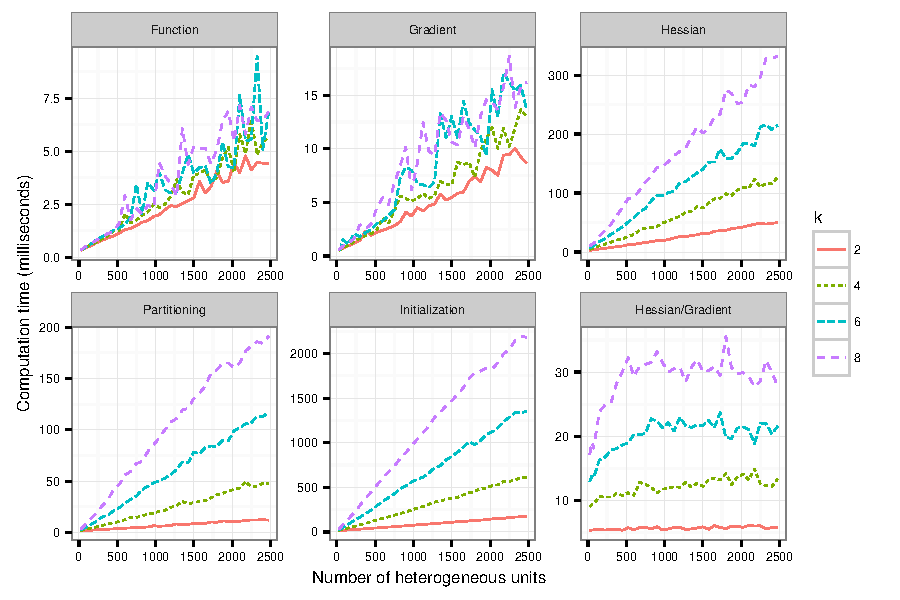
\includegraphics{fig_timings}
  \caption{Run times for sparse Hessian computation.}
  \label{fig:timing}
\end{figure}

Computation times
for the function and gradient, as well as the setup and
partitioning times for the \class{sparseHessianFD} object, grow
linearly with the number of heterogenous units.  The time
for the Hessian grows linearly as well, and that might be partially
surprising.  We saw in Section~\ref{sec:coloring} that adding
additional heterogeneous units in a hierarchical model does not
increase the number of required gradient evaluations.  So we might
think that the time
to compute a Hessian should not increase with $N$ \emph{at all}.  The
reason it does is that each gradient evaluation takes longer.
Nevertheless, we can conclude that the
\pkg{sparseHessianFD} algorithms are quite efficient and scalable for
hierarchical models.

\FloatBarrier
\bibliography{sparseHessianFD}

\end{document}
